\documentclass[main.tex]{subfiles}

\begin{document}

\subsection{Primo esercizio}

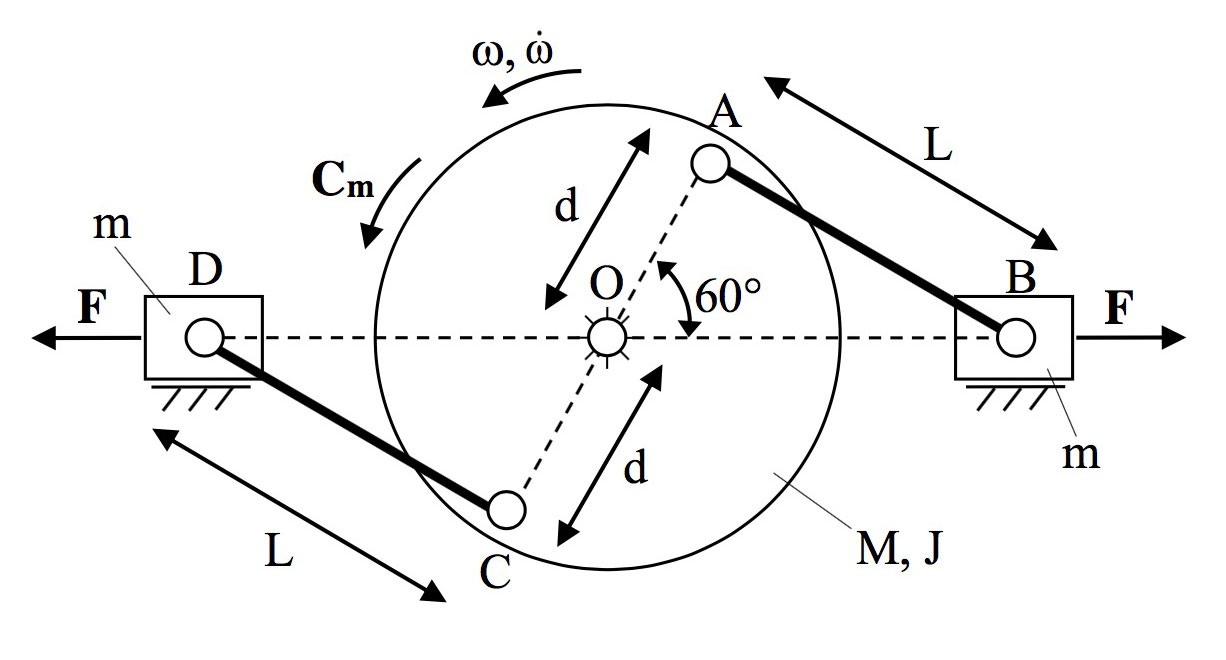
\includegraphics[width=\textwidth]{2014-1009-1.jpg}

\[
	d =0.1\,m \quad
	L = d\sqrt{3} \quad
	M = 4\,kg \quad
	J = 0.03\,kgm^2 \quad
\]
\[
	m = 1\,kg \quad
	\omega = 50\,rad/s  \quad
	\dot{\omega} = 5\,rad/s^2 \quad
	F = 100\,N \quad
\]

Il sistema rappresentato in figura è posto nel piano verticale. Il disco, avente massa $M$ e momento d'inerzia $J$ è incernierato a terra in O, mentre in A e C sono incernierate due aste di lunghezza $L$, con massa e momento di inerzia trascurabili. Agli estremi delle aste sono incernierati due corsoi, entrambi di massa $m$, vincolati a scorrere lungo due guide orizzontali e ai quali sono applicate due forze $F$ aventi lo stesso modulo e la stessa direzione, ma versi opposti. Si consideri trascurabile l’attrito tra i due corsoi e le rispettive guide. Come indicato in figura, sul disco AB agisce una coppia $C_m$.

Nota la geometria del sistema e assegnate la velocità e l’accelerazione angolare del disco si chiede di calcolare:

\begin{enumerate}
\item La velocità e l'accelerazione dei B e D.
\item La coppia $C_m$ necessaria per garantire la condizione di moto assegnata.
\end{enumerate}

\clearpage

\subsection{Soluzione primo esercizio (non verificata)}

\subsubsection{Osservazioni}

\begin{enumerate}
\item In ogni dato momento, $a_D = -a_B$ e $v_D = -v_B$.
\end{enumerate}

\subsubsection{Primo punto}

\paragraph{Definizione dell'equazione di chiusura} sicché il sistema risulta simmetrico lungo la bisettrice $y = -x$ possiamo trattare uno dei due lati singolarmente, attendendo un risultato analogo sulla parte opposta, calcolabile cambiando di segno. Definisco quindi l'equazione di chiusura dell'esercizio come:

\[
	(O-A) + (A-B) = (O-B)
\]

\paragraph{Spostamento} Dopo aver definito le seguenti variabili, $d = OA$, $L = AB$, $b = OB$, $\alpha$ l'angolo interno in O e $\beta$ l'angolo interno in B, vado a scrivere l'espressione dello spostamento con il metodo dei numeri complessi.

\[
	de^{i\alpha} + Le^{i\beta} = b
\]

Scompongo cartesianamente ed ottengo:

\[
	\begin{cases}
		d\sin\alpha + L\sin\beta = 0\\
		d\cos\alpha + L\cos\beta = b\\
	\end{cases}
	\Longrightarrow
	\begin{cases}
		\beta = \arcsin\left (-\dfrac{d\sin\alpha}{L}\right ) = -\dfrac{\pi}{3}\,rad\\
		b = d\cos\alpha + L\cos\beta = 0.2\,m\\
	\end{cases}
\]

I risultati ottenuti sono in linea con la geometria illustrata, e mostrano ancor meglio, se non fosse già chiaro, che i segmenti OAB danno origine ad un triangolo rettangolo.

\paragraph{Velocità} Derivo lo spostamento ed ottengo la velocità, ricordando che i termini variabili sono $\alpha$, $\beta$ e $b$:

\[
	d\dot{\alpha}e^{i \left (\dfrac{\pi}{2} + \alpha\right )} + L\dot{\beta}e^{i \left (\dfrac{\pi}{2} + \beta\right )} = \dot{b}
\]

Scompongo cartesianamente, ricordando che $\dot{\alpha} = \omega$:

\[
\begin{cases}
	d\omega\cos(\alpha) + L\dot{\beta}\cos(\beta) = 0\\
	-d\omega\sin(\alpha) - L\dot{\beta}\sin(\beta) = \dot{b}
\end{cases}
\Longrightarrow
\begin{cases}
	\dot{\beta} = -\dfrac{d\omega\cos(\alpha)}{L\cos(\beta)} = -16.6\,rad/s\\
	\dot{b} =-d\omega\sin(\alpha) - L\dot{\beta}\sin(\beta) = -5.76\,m/s
\end{cases}
\]

\paragraph{Accelerazione} Derivo nuovamente ed ottengo l'accelerazione, prestando attenzione che i termini variabili sono $\alpha$, $\beta$, $\dot{b}$, $\dot{\alpha}$ e $\dot{\beta}$:

\[
	d\ddot{\alpha}e^{i \left (\dfrac{\pi}{2} + \alpha\right )} - d\dot{\alpha}^2e^{i\alpha} + L\ddot{\beta}e^{i \left (\dfrac{\pi}{2} + \beta\right )} - L\dot{\beta}^2e^{i\beta}= \ddot{b}
\]

Scompongo cartesianamente, ricordando che $\ddot{\alpha} = \dot{\omega}$:

\[
	\begin{cases}
	d\dot{\omega}\cos\alpha - d\omega^2\sin\alpha + L\ddot{\beta}\cos\beta - L\dot{\beta}^2\sin\beta = 0\\
	-d\dot{\omega}\sin\alpha - d\omega^2\cos\alpha - L\ddot{\beta}\sin\beta - L\dot{\beta}^2\cos\beta = \ddot{b}\\
	\end{cases}
\]
\[
	\begin{cases}
	\ddot{\beta} = \dfrac{d\omega^2\sin\alpha + L\dot{\beta}^2\sin\beta -d\dot{\omega}\cos\alpha}{L\cos\beta} = 1282.6\,rad/s^2 \\
	\ddot{b} = -d\dot{\omega}\sin\alpha - d\omega^2\cos\alpha - L\ddot{\beta}\sin\beta - L\dot{\beta}^2\cos\beta = -55.7\,m/s^2\\
	\end{cases}
\]

Riassumendo, $v_b = -v_d = -5.76\,m/s$ e $a_b = -a_d = -55.7\,m/s^2$

\subsubsection{Secondo punto}

Uso l'equazione del bilancio di potenze per andare a calcolare il valore assunto di $C_m$ nella corrente condizione di moto.

\[
	\sum W_i = \dfrac{dE_c}{dt}
\]

\paragraph{Energia cinetica totale} Per determinare l'energia cinetica totale, vado a considerare tutte le masse in movimento rotatorio o traslatorio, in questo frangente tutte.

\[
	E_c = \dfrac{1}{2}J\omega^2 + \dfrac{1}{2}mv_b^2 + \dfrac{1}{2}mv_d^2 = \dfrac{1}{2}J\omega^2 + mv^2
\]

\paragraph{Derivo energia cinetica}

\[
	\dfrac{dE_c}{dt} = J\omega\dot{\omega} + 2mva
\]

\paragraph{Potenza totale} Per determinare la potenza totale, vado a considerare tutte le forze e le coppie che vengono applicate a corpi in movimento.

Essendo sul piano verticale, vanno considerate le forze peso, ma in questo caso tutti i baricentri di corpi rotanti corrispondono con il centro geometrico e tutti i corpi sono vincolati a terra, per cui ad ogni forza peso corrisponde una forza normale uguale ed opposta.

Non sono presenti attriti di alcun genere, nè volventi, nè dinamici, nè statici.

L'unica forza da prendere in considerazione è la forza $\vec{F}$, che agisce sui due corsoi. Ogni corsoio, possiede una velocità con direzione uguale ed opposta alla forza che vi viene applicata, per cui tutte esse vanno a formare un angolo di $\pi$ con il vettore $\vec{v}$ corrispondente.

La coppia $C_m$, infinite, viene data dal testo come orientata nella stessa direzione di $\omega$.

\[
	\sum W_i =  \vec{C}_m\bullet\vec{\omega} + \vec{F}_D\bullet\vec{v}_D +  \vec{F}_B\bullet\vec{v}_B
\]

Risolvo il prodotto scalare sostituendo con la formula nota: $\vec{F}\bullet\vec{v} = |F||v|\cos\theta$ con $theta$ definito come l'angolo compreso tra i due vettori:

\[
	\sum W_i = C_m\omega\cos0 2Fv\cos\pi = C_m\omega-2Fv
\]

\paragraph{Uso il bilancio delle potenze}

\begin{equation}
	C_m\omega-2Fv =  J\omega\dot{\omega} + 2mva
\end{equation}

\begin{equation}
	C_m\omega =  2Fv + J\omega\dot{\omega} + 2mva
\end{equation}

\begin{equation}
	C_m = \dfrac{2Fv + J\omega\dot{\omega} + 2mva}{\omega}
\end{equation}

Risolvo numericamente ed ottengo:

\begin{equation}
	C_m = 36\,Nm
\end{equation}

\end{document}